% Escolha: Portugues ou Ingles ou Espanhol.
% Para a versão final do texto, após a defesa, acrescente Final:

\documentclass[Ingles]{ic-tese-v3}
%\documentclass[Portugues,Final]{ic-tese-v3}

\usepackage[latin1,utf8]{inputenc}

% Para acrescentar comentários ao PDF descomente:
\usepackage
%  [pdfauthor={nome do autor},
%   pdftitle={titulo},
%   pdfkeywords={palavra-chave, palavra-chave},
%   pdfproducer={Latex with hyperref},
%   pdfcreator={pdflatex}]
{hyperref}

\usepackage{hyperref}
\usepackage{ae}
\usepackage{indentfirst}
\usepackage{colortbl}
\usepackage{amssymb,amsmath,graphicx,fancyhdr,psfrag,tabularx,float,textcomp,fancybox,amsfonts}
\usepackage{algorithmic}
\usepackage{color}
\usepackage{rotating}
\usepackage{epsfig}
\usepackage{ifthen}
\usepackage{lscape}
\usepackage{array}
\usepackage{forest}
\usepackage{setspace}
\usepackage{xcolor}
\usepackage{lipsum}
\usepackage{pbox}
\usepackage{multirow}
\RequirePackage{multicol}
\usepackage{adjustbox}
\usepackage{caption}
\usepackage{longtable}
\usepackage[autostyle]{csquotes}
\usepackage{comment}
\usepackage{enumerate}
\usepackage{manyfoot}
\usepackage{listings}
\usepackage{arydshln}
\usetikzlibrary{arrows,shapes}
\usepackage{pgf-pie}
\usepackage{bbding}
\usepackage{url}
\usepackage{verbatim}
\usepackage{booktabs}
\usepackage{siunitx}
\usepackage{makecell}
\usepackage{pifont}
\usepackage{natbib}
\usepackage[noabbrev,nameinlink,capitalise]{cleveref}
\usepackage{eqparbox}
\usepackage{enumitem}

% algorithms
\usepackage[english,ruled,lined,linesnumbered]{algorithm2e} % Escrever algoritmos

% images
\usepackage{tikz}
\usepackage{pgf}
\usepackage{pgfplots}
\usepackage{geometry}
\usepackage{subcaption}

% fonts
\usepackage[utf8]{inputenc}
\usepackage[english]{babel}
\usepackage{amsthm}

% math
\usepackage{calc}% http://ctan.org/pkg/calc
\usepackage[T1]{fontenc}
\usepackage{theoremref}

% read data
\usepackage{readarray,tokcycle}

\SetKwInput{Input}{Input}%
\SetKwInput{Output}{Output}%

\newtheorem{property}{Property}
\newtheorem{proposition}{Proposition}
\newtheorem{definition}{Definition}

\newcommand{\z}{$\bullet$}
\newcommand{\drawBlock}[3]{
  \draw [fill=#3, draw = white] (#1) \foreach \v [count=\i] in #2 {
    \ifnum\i>1
      -- (\v)
    \fi
  } -- cycle;
}
\newcommand{\drawArcs}[3]{
  \foreach \i in {1,...,#2}{
    \draw [#3] (#1[\i,1]) -- (#1[\i,2]);
  }
}
\newcommand{\drawArcsBend}[3]{
  \foreach \i in {1,...,#2}{
    \draw [#3] (#1[\i,1]) to [bend right=3] (#1[\i,2]);
  }
}

%%%%%%%%%%%%%%%%%%%%%%%%%%%%%%%%%%%%
%%%%%%%%%% Tikz settings %%%%%%%%%%%
%%%%%%%%%%%%%%%%%%%%%%%%%%%%%%%%%%%%

\usetikzlibrary{arrows.meta,arrows}
\usetikzlibrary{arrows,positioning,automata,shadows,fit,shapes,calc,shapes.geometric}
\usetikzlibrary{decorations.pathmorphing}
\tikzset{triangle_black/.style={regular polygon, regular polygon sides=3, minimum size=0.3cm, fill=black}}
\tikzset{triangle/.style={regular polygon, regular polygon sides=3, minimum size=0.3cm, fill=white}}
\tikzset{square/.style={regular polygon, regular polygon sides=4, minimum size=0.3cm, fill=white}}
\tikzset{circufe/.style={circle,draw, minimum size=0.2cm, fill=white}}
\tikzset{raio/.style={circle,draw, minimum size=1.45cm, fill=white}} 
\tikzset{circle_new/.style={circle,draw, minimum size=0.2cm, fill=white}}   
\geometry{
  a4paper,
%  total={170mm,257mm},
  left=1in,
  top=1in,
  bottom=1in,
  right=1in
}

\usepackage{glossaries}

\makeglossaries
\newacronym{ew}{EW}{Epidemiological Week}
\newacronym{ml}{ML}{Machine Learning}
\newacronym{gis}{GIS}{Geographic Information System}
\newacronym{paho}{PAHO}{Pan American Health Organization}
\newacronym{who}{WHO}{World Health Organization}
\newacronym{or}{OR}{Operations Research}
\newacronym{osm}{OSM}{Open Street Maps}
\newacronym{mabs}{MABS}{Multi-Agent-Based Simulation}
\newacronym{ode}{ODE}{Ordinary Differential Equations}
\newacronym{darp}{Dengue-PARP}{Dengue Prize-collecting Arc Routing Problem}
\newacronym{sinan}{SINAN}{Information System for Notifiable Disease}
\newacronym{ibge}{IBGE}{Brazilian Institute of Geography and Statistics}
\newacronym{mae}{MAE}{Mean Absolute Error}
\newacronym{vrp}{VRP}{Vehicle Routing Problem}
\newacronym{arp}{ARP}{Arc Routing Problem}
\newacronym{cbrp}{CBRP}{City Block Routing Problem}
\newacronym{ilp}{ILP}{Integer Linear Programming}
\newacronym{milp}{MILP}{Mixed Interger Linear Programming}
\newacronym{mtz}{MTZ}{Miller-Tucker-Zemlin}
\newacronym{scbrp}{SCBRP}{Stochastic City Block Routing Problem}
\newacronym{lr}{LR}{Lagrangean Relaxation}
\newacronym{lpp}{LPP}{Lagrangian Primal Problem}
\newacronym{ldp}{LDP}{Lagrangian Dual Problem}



\begin{document}

% Escolha entre autor ou autora:
\autor{Carlos Victor Dantas Araújo}
%\autora{Nome da Autora}

% Sempre deve haver um título em português:
% \titulo{Dengue Control}

% Se a língua for o inglês ou o espanhol defina:
\title{Dengue Control}

% Escolha entre orientador ou orientadora. Inclua os títulos acadêmicos:
\orientador{Prof. Dr. Fábio Luiz Usberti}
%\orientadora{Profa. Dra. Nome da Orientadora}

% Escolha entre coorientador ou coorientadora, se houver.  Inclua os títulos acadêmicos:
%\coorientador{Prof. Dr. Eng. Lic. Nome do Co-Orientador}
%\coorientadora{Profa. Dra. Eng. Lic. Nome da Co-Orientadora}

% Escolha entre mestrado ou doutorado:
% \mestrado
\doutorado

% Se houve cotutela, defina:
%\cotutela{Universidade Nova de Plutão}

\datadadefesa{22}{09}{2025}

% Para a versão final defina:
%\avaliadorA{Prof. Dr. Primeiro Avaliador}{Instituição do primeiro avaliador}
%\avaliadorB{Profa. Dra. Segunda Avaliadora}{Instituição da segunda avaliadora}
%\avaliadorC{Dr. Terceiro Avaliador}{Instituição do terceiro avaliador}
%\avaliadorD{Prof. Dr. Quarto Avaliador}{Instituição do quarto avaliador}
%\avaliadorE{Prof. Dr. Quinto Avaliador}{Instituição do quinto avaliador}
%\avaliadorF{Prof. Dr. Sexto Avaliador}{Instituição do sexto avaliador}
%\avaliadorG{Prof. Dr. Sétimo Avaliador}{Instituição do sétimo avaliador}
%\avaliadorH{Prof. Dr. Oitavo Avaliador}{Instituição do oitavo avaliador}


% Para incluir a ficha catalográfica em PDF na versão final, descomente e ajuste:
%\fichacatalografica{arquivo.pdf}


% Este comando deve ficar aqui:
\paginasiniciais


% Se houver dedicatória, descomente:
%\prefacesection{Dedicatória}
%A dedicatória deve ocupar uma única página.


% Se houver epígrafe, descomente e edite:
% \begin{epigrafe}
% {\it
% Vita brevis,\\
% ars longa,\\
% occasio praeceps,\\
% experimentum periculosum,\\
% iudicium difficile.}
%
% \hfill (Hippocrates)
% \end{epigrafe}


% Agradecimentos ou Acknowledgements ou Agradecimientos
\prefacesection{Acknowledgements}
Os agradecimentos devem ocupar uma única página.


% Sempre deve haver um resumo em português:
\begin{resumo}
	O resumo deve ter no máximo 500 palavras e deve ocupar uma única página.
\end{resumo}


% Sempre deve haver um abstract:
\begin{abstract}
	The abstract must have at most 500 words and must fit in a single page.
\end{abstract}


% Se houver um resumo em espanhol, descomente:
%\begin{resumen}
% A mesma regra aplica-se.
%\end{resumen}


% A lista de figuras é opcional:
\listoffigures

% A lista de tabelas é opcional:
\listoftables

% A lista de abreviações e siglas é opcional:
% \prefacesection{Lista de Abreviações e Siglas}
\printglossary[type=\acronymtype]
% \printglossaries

% A lista de símbolos é opcional:
% \prefacesection{Lista de Símbolos}

% Quem usa o pacote nomencl pode incluir:
% \renewcommand{\nomname}{Lista de Abreviações e Siglas}
% \printnomenclature[3cm]


% O sumário vem aqui:
\tableofcontents


% E esta linha deve ficar bem aqui:
\fimdaspaginasiniciais

\chapter{Introduction}\label{chp:introduction}

Dengue is a mosquito-borne viral infection primarily transmitted by \textit{Aedes aegypti} mosquitoes. The disease, caused by any of the four distinct serotypes of the Dengue virus, poses a significant global public health challenge~\citep{shepard:2016}. Environmental and ecological changes, such as rising temperatures, increased urbanization, and changing precipitation patterns, have expanded the range of \textit{Aedes aegypti}, contributing to the greater geographic spread of Dengue. Since its emergence in the late 18\textsuperscript{th} century in Asia and the Pacific, Dengue has become endemic in many regions, with approximately half of the world's population currently living in areas at risk~\citep{fares:2015,negreiros-2020}. Factors such as rapid population growth, unplanned urban development, inadequate sanitation, and healthcare inequality play a central role in the persistence and resurgence of dengue.

In 2021, the Pan American Health Organization (PAHO) reported more than $1.3$ million cases of arboviral diseases in the Americas, with Dengue alone accounting for $1.1$ million cases, approximately 89\% of the total. Despite occupying about 45\% of Latin America's landmass, Brazil contributed to more 60\% of Dengue cases in the region~\citep{BardachEtal2019}. In 2022, Brazil reported 2,363,490 Dengue cases, representing 84.11\% of global cases and 99.65\% of those in South America; 1,210,760 of these were laboratory confirmed. 

In the last year, 2024, Brazil reported approximately $10.239.883$ cases of Dengue, accounting for $78,62\%$ of the world's cases and $92,10\%$ of the South American cases. Of the reported cases, $10.231.692$ were confirmed in the laboratory, $8.191$ were classified as severe, and $6.161$ resulted in death. According to the epidemiological report of the Brazil Health Departments up to April 20, 2024, more than 11 states and 465 cities declared a state of emergency~\citep{health-dp-1}. By 28 February 2025, Brazil had reported $662.224$ cases of Dengue, which represents $86.43\%$ of the World's cases. Figure~\ref{picture:dengue_reported_cases_graphic}
displays a graph that shows the number of Dengue cases in the world, South America, and Brazil from 1980 to 2024.

% TOPDO: UPDATE GRAPH AND TEXT
\begin{figure}[!ht]
    \centering
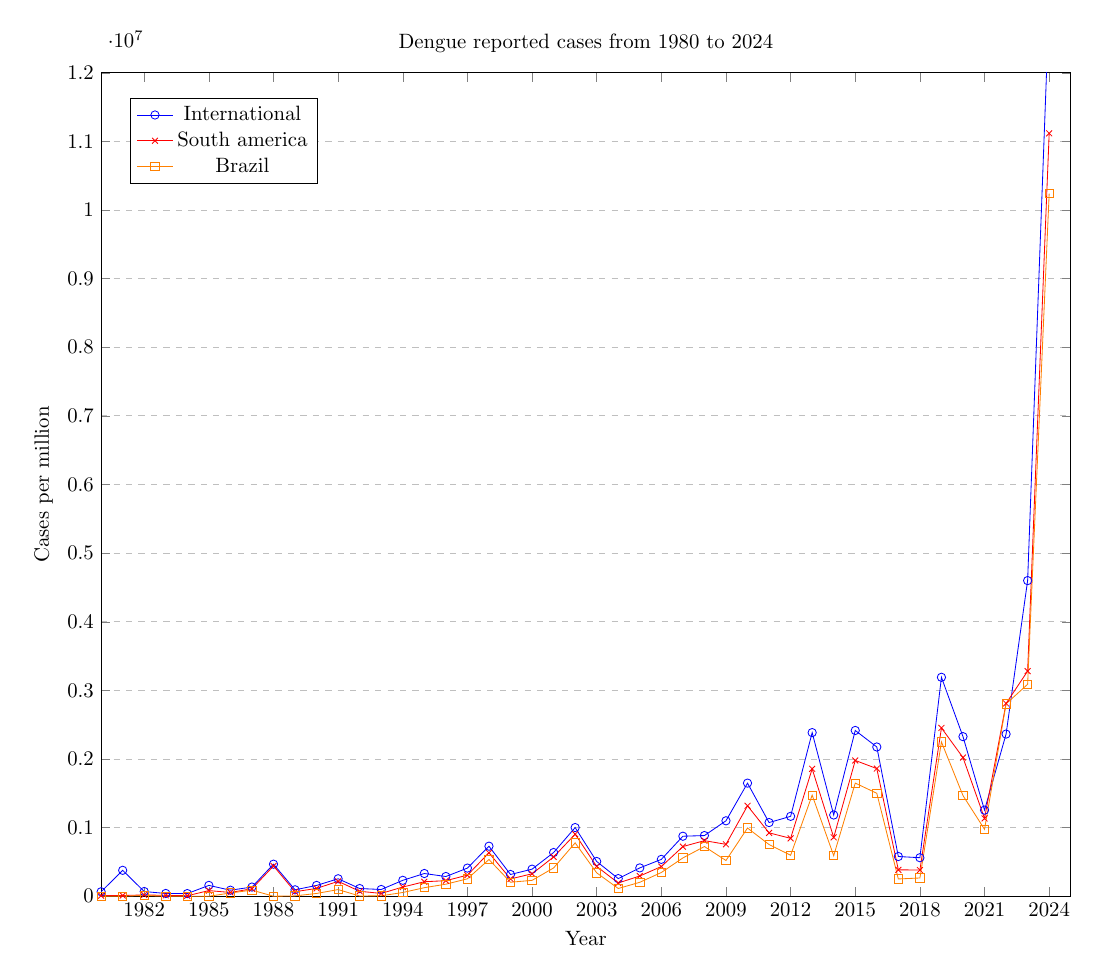
\begin{tikzpicture}[>=latex, scale=.75]
  \begin{axis}[
    width = {18cm},
    title={Dengue reported cases from 1980 to 2024},
    xlabel={Year},
    ylabel={Cases per million},
    xmin=1980, xmax=2025,
    ymin=0, ymax=12000000,
    xtick={1982, 1985, 1988, 1991, 1994, 1997, 2000, 2003, 2006, 2009, 2012, 2015, 2018, 2021, 2024},
    xticklabels={1982, 1985, 1988, 1991, 1994, 1997, 2000, 2003, 2006, 2009, 2012, 2015, 2018, 2021, 2024},
    legend pos=north west,
    ymajorgrids=true,
    grid style=dashed,
    ]

    \addplot[
      color=blue,
      mark=o,
      ]
      plot coordinates {
        (1980, 65523)
        (1981, 377916)
        (1982, 68892)
        (1983, 40544)
        (1984, 38904)
        (1985, 158193)
        (1986, 88093)
        (1987, 134013)
        (1988, 467386)
        (1989, 94179)
        (1990, 157662)
        (1991, 254749)
        (1992, 112567)
        (1993, 98598)
        (1994, 232051)
        (1995, 331417)
        (1996, 287519)
        (1997, 410392)
        (1998, 729425)
        (1999, 317158)
        (2000, 394857)
        (2001, 636977)
        (2002, 1001073)
        (2003, 506726)
        (2004, 257251)
        (2005, 413122)
        (2006, 537412)
        (2007, 874750)
        (2008, 884334)
        (2009, 1099742)
        (2010, 1648569)
        (2011, 1073990)
        (2012, 1164366)
        (2013, 2384803)
        (2014, 1184045)
        (2015, 2416018)
        (2016, 2175409)
        (2017, 579027)
        (2018, 561689)
        (2019, 3190778)
        (2020, 2326115)
        (2021, 1254648)
        (2022, 2363490)
        (2023, 4600086)
        (2024, 13036652)
      };
    \addlegendentry{International}

    \addplot[
      color=red,
      mark=x,
      ]
      plot coordinates {
        (1980, 9003)
        (1981, 10861)
        (1982, 19034)
        (1983, 12925)
        (1984, 7560)
        (1985, 82273)
        (1986, 55248)
        (1987, 108955)
        (1988, 441382)
        (1989, 65803)
        (1990, 114431)
        (1991, 217077)
        (1992, 72319)
        (1993, 41250)
        (1994, 134342)
        (1995, 211396)
        (1996, 226960)
        (1997, 307625)
        (1998, 632804)
        (1999, 252762)
        (2000, 326846)
        (2001, 572876)
        (2002, 903891)
        (2003, 434264)
        (2004, 193334)
        (2005, 294943)
        (2006, 432661)
        (2007, 724077)
        (2008, 810134)
        (2009, 756755)
        (2010, 1317801)
        (2011, 923793)
        (2012, 843840)
        (2013, 1857228)
        (2014, 857983)
        (2015, 1978921)
        (2016, 1860466)
        (2017, 385076)
        (2018, 382243)
        (2019, 2453060)
        (2020, 2021272)
        (2021, 1134555)
        (2022, 2809818)
        (2023, 3280394)
        (2024, 11118085)
      };
    \addlegendentry{South america}

    \addplot[
      color=orange,
      mark=square,
      ]
      plot coordinates {
        (1980, 0)
        (1981, 0)
        (1982, 12000)
        (1983, 0)
        (1984, 0)
        (1985, 0)
        (1986, 47367)
        (1987, 89393)
        (1988, 190)
        (1989, 5334)
        (1990, 40642)
        (1991, 97209)
        (1992, 3501)
        (1993, 6915)
        (1994, 54453)
        (1995, 124775)
        (1996, 175749)
        (1997, 254074)
        (1998, 535283)
        (1999, 204131)
        (2000, 231412)
        (2001, 412388)
        (2002, 778037)
        (2003, 341189)
        (2004, 112851)
        (2005, 203356)
        (2006, 345922)
        (2007, 558413)
        (2008, 724427)
        (2009, 520660)
        (2010, 994158)
        (2011, 753487)
        (2012, 597450)
        (2013, 1473645)
        (2014, 591080)
        (2015, 1649008)
        (2016, 1500535)
        (2017, 252054)
        (2018, 265934)
        (2019, 2248570)
        (2020, 1467142)
        (2021, 975474)
        (2022, 2803567)
        (2023, 3088723)
        (2024, 10239883)
      };
      \addlegendentry{Brazil}
  \end{axis}
\end{tikzpicture}
\caption{Dengue reported cases from 1980 to 2024~\citep{paho-1}.}
\label{picture:dengue_reported_cases_graphic}
\end{figure}

The disease imposes substantial social and economic burdens, affecting not only the health and well-being of individuals but also the broader economic productivity and healthcare system. The financial impact of Dengue in Brazil is profound, for example, annual expenditures on Dengue prevention and control exceed BRL $1.6$ billion~\citep{negreiros-2020}. The direct costs include healthcare expenses for hospitalization, medical treatment, and public health campaigns aimed at controlling mosquito populations~\citep{negreiros:2008}. Indirect costs, such as lost productivity due to illness and the long-term effects of severe Dengue cases, add to the financial strain. Moreover, the social consequences are equally alarming, with communities enduring the disruption of daily life, increased anxiety over disease outbreaks, and the loss of lives. 

Despite the severity of the situation, most Brazilian municipalities continue to make crucial decisions in combating Dengue without the support of advanced computational tools~\citep{brasil-dept-helth:2009}. The current approach is largely reactive, relying on traditional mosquito control methods, including eliminating adult mosquitoes, their breeding sites and public health interventions. These actions are often insufficient to address the complexity and scale of the problem. This lack of computational support means that decisions regarding resource allocation, strategic planning, and the deployment of interventions are not optimized, leading to possible inefficiencies and potentially exacerbating the spread of the disease~\citep{forbes-2002,xie-2015,rais-2011}.

The most common approach to combating Dengue spread is employing chemical control methods, such as insecticides, which manage the mosquito population in both the larval and adult stages~\citep{brasil-dept-helth:2009}. The \gls{who} provides technical and operational standards for pesticide experts to ensure the safe use of insecticides in public health. These standards specify the active ingredients and dosages for various treatments. It is essential to use insecticides carefully and responsibly in vector control activities, as indiscriminate use can have significant environmental impacts and contribute to developing resistance in mosquitoes~\citep{WHO2009,WHO2020}.

During disease outbreaks, emergency responses in urban areas usually involve the dispatch of spraying vehicles to apply insecticides see Figure~\ref{fig:nebulizer}. As a result, health authorities with limited budgets must make two key decisions: first, selecting which city blocks should receive insecticide spraying to maximize vector suppression; and second, optimizing vehicle routes to ensure the efficient use of available resources. In this context, there is a clear and urgent need to integrate computational models and decision-support systems into Dengue control strategies. Such tools can help municipalities better predict outbreaks, optimize resource use, and implement more effective mosquito control measures. 

\begin{figure}[!ht]
  \centering
    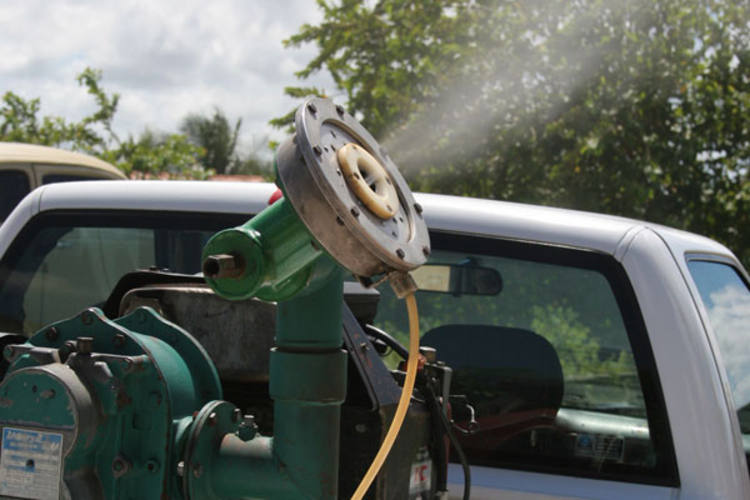
\includegraphics[scale=0.5]{images/fumace.jpg}
    \caption{Nebulizer equipment attached to vehicle \citep{fumace-2022}.}
    \label{fig:nebulizer}
\end{figure}

The sprayed insecticide has no residual  effect and it is strongly influenced by wind  and obstacles  along the  streets. The  best effect  is achieved  when the densest  insecticide cloud  is at  a distance  of at  most 100  meters from  the equipment~\citep{brasil-dept-helth:2009}.  As this  distance  is  crossed, the  effectiveness  decreases, as a consequence of droplet drift influenced by factors of the environment. The cloud dispersion is illustrated in Figure~\ref{fig:dispersion}.

\begin{figure}[!ht]
  \centering
  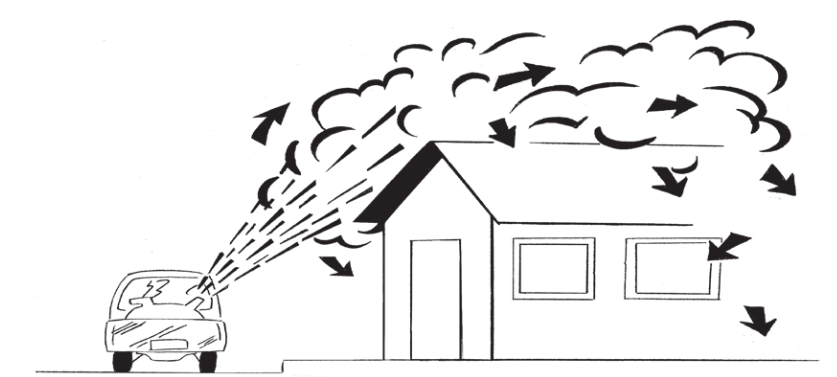
\includegraphics[scale=0.4]{images/cloud-dispersion.png}
  \caption{Cloud dispersion of the application \citep{brasil-dept-helth:2009}.}
  \label{fig:dispersion}
\end{figure}

Insecticide application instructions are generally based on ideal topology conditions, locality structure, and favorable
winds. The operation is often affected by unpaved roads, the presence of high
walls,  and  high   vegetation,  in  addition  to   headwinds.  The application methodology must consider these limitations to obtain a good impact on the
vector population. The vehicle must travel around each block before starting the
next one, as shown in Figure \ref{fig:travel-pattern}.

\begin{figure}[!ht]
  \centering
  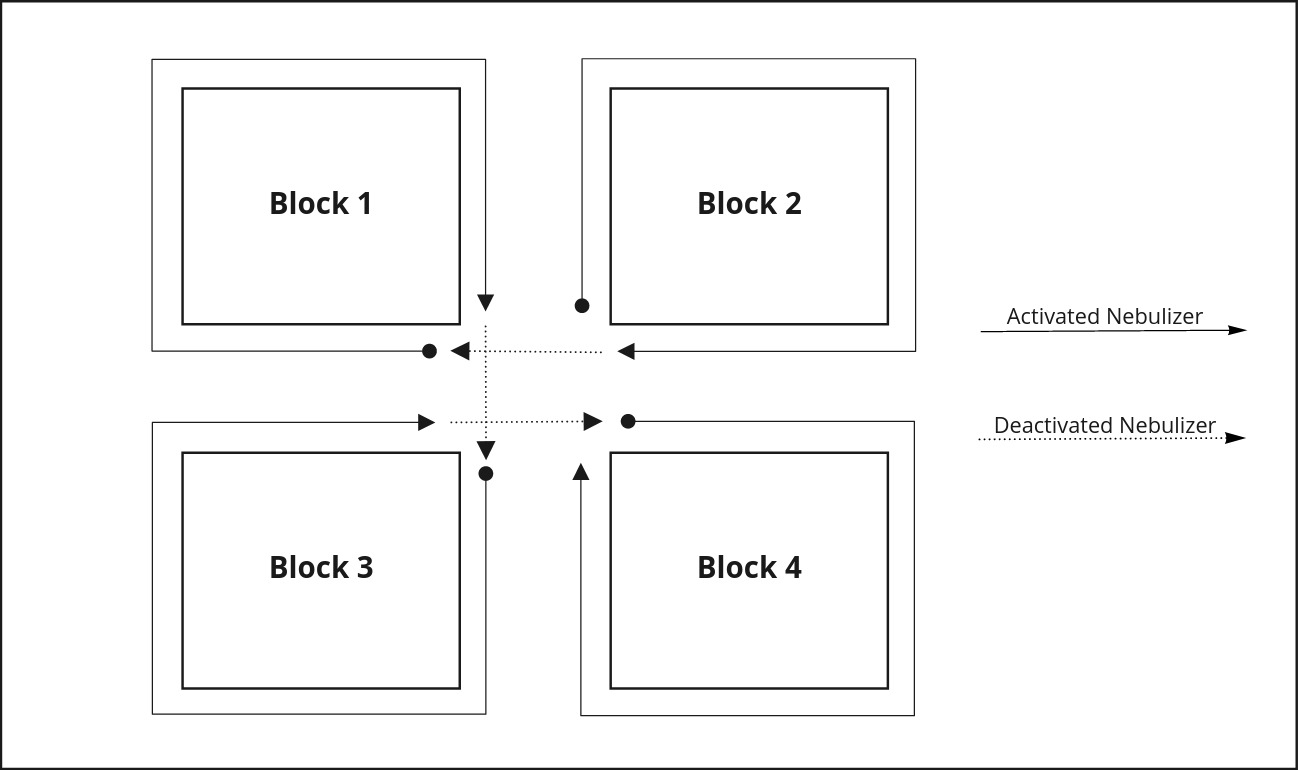
\includegraphics[scale=0.25]{images/visit-pattern.jpg}
  \caption{Vehicle pattern with nebulizer \cite{brasil-dept-helth:2009}.}
  \label{fig:travel-pattern}
\end{figure}

Figure~\ref{fig:ex1} illustrates an example of an input graph and a corresponding CBRP feasible solution. In Figure~\ref{subfig:a}, the circles represent the graph nodes, while the labels from A to H indicate the blocks computed by the method described in Section~\ref{sec:data}. Figure~\ref{subfig:b} depicts a feasible solution to the CBRP. In this solution, 
the nodes used in the route are marked as squares (nodes 4, 5, 3, and 9). Squares with a double border denote nodes that act as starting points to serve at least one block. The served blocks are represented with dashed borders and colored to match the corresponding route node: node 4 (blue) serves blocks A and B, node 5 (red) serves D and F, node 3 does not serve any block, and node 9 (teal) serves block H.
%
\begin{figure}[!ht]
\begin{subfigure}{.5\textwidth}
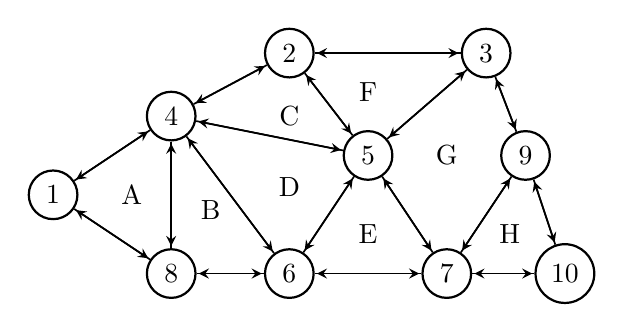
\begin{tikzpicture}[
            > = stealth, % arrow head style
            shorten > = 0.8pt, % don't touch arrow head to node
            auto,
            node distance = 1cm, % distance between nodes
            semithick % line style
        ]

        \tikzstyle{every state}=[
            draw = black,
            thick,
            fill = white,
            minimum size = 5mm
        ]

        \node[state] (a) [at={(-1, -0.5)}]{$1$};
        \node[state] (b) [at={(2,1.3)}] {$2$};
        \node[state] (c) [at={(4.5,1.3)}] {$3$};
        \node[state] (d) [at={(0.5, 0.5)}] {$4$};
        \node[state] (e) [at={(3, 0)}] {$5$};
        \node[state] (f) [at={(2,-1.5)}] {$6$};
        \node[state] (g) [at={(4,-1.5)}] {$7$};
        \node[state] (i) [at={(0.5,-1.5)}] {$8$};
        \node[state] (j) [at={(5,0)}] {$9$};
        \node[state] (k) [at={(5.5,-1.5)}] {$10$};
        % Blocks
        \node[state, draw = white, right of = a] {A};
        \node[state, draw = white, right of = i, yshift=0.8cm, xshift=-0.5cm] {B};
        \node[state, draw = white, below of = b, yshift=0.2cm] {C};
        \node[state, draw = white, left of = e, yshift=-0.4cm] {D};
        \node[state, draw = white, below of = e] {E};
        \node[state, draw = white, right of = b, yshift=-0.5cm] {F};
        \node[state, draw = white, right of = e] {G};
        \node[state, draw = white, below of = j, xshift=-0.2cm] {H};
        
        
        \path[->] (a) edge node {} (d); 
        \path[->] (d) edge node {} (a); 
        \path[->] (i) edge node {} (a);
        \path[->] (a) edge node {} (i);
        \path[->] (b) edge node {} (d);
        \path[->] (d) edge node {} (b);
        \path[->] (b) edge node {} (c);
        \path[->] (c) edge node {} (b);
        \path[->] (c) edge node {} (e);
        \path[->] (e) edge node {} (c);
        \path[->] (e) edge node {} (f);
        \path[->] (f) edge node {} (e);
        \path[->] (d) edge node {} (i);
        \path[->] (i) edge node {} (d);
        \path[->] (d) edge node {} (e);
        \path[->] (e) edge node {} (d);
        \path[->] (d) edge node {} (f);
        \path[->] (f) edge node {} (d);
        \path[->] (e) edge node {} (g);
        \path[->] (g) edge node {} (e);
        \path[->] (c) edge node {} (j);
        \path[->] (j) edge node {} (c);
        \path[->] (i) edge node {} (f);
        \path[->] (f) edge node {} (i);
        \path[->] (j) edge node {} (k);
        \path[->] (k) edge node {} (j);
        \path[->] (j) edge node {} (g);
        \path[->] (g) edge node {} (j);
        \path[->] (e) edge node {} (b);
        \path[->] (b) edge node {} (e);
        \path[->] (f) edge node {} (g);
        \path[->] (g) edge node {} (f);
        \path[->] (g) edge node {} (k);
        \path[->] (k) edge node {} (g);
        
\end{tikzpicture}
\subcaption{\label{subfig:a} Initial graph and blocks.}
\end{subfigure}
% Segunda figura
\begin{subfigure}{.5\textwidth}
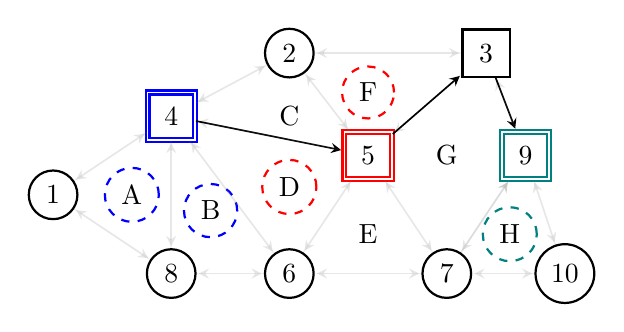
\begin{tikzpicture}[
            > = stealth, % arrow head style
            shorten > = 0.8pt, % don't touch arrow head to node
            auto,
            node distance = 1cm, % distance between nodes
            semithick % line style
        ]

        \tikzstyle{every state}=[
            draw = black,
            thick,
            fill = white,
            minimum size = 6mm
        ]

        \node[state] (a) [at={(-1, -0.5)}]{$1$};
        \node[state] (b) [at={(2,1.3)}] {$2$};
        \node[state, rectangle] (c) [at={(4.5,1.3)}] {$3$};
        \node[state, rectangle, double, draw=blue] (d) [at={(0.5, 0.5)}] {$4$};
        \node[state, rectangle, double, draw=red] (e) [at={(3, 0)}] {$5$};
        \node[state] (f) [at={(2,-1.5)}] {$6$};
        \node[state] (g) [at={(4,-1.5)}] {$7$};
        \node[state] (i) [at={(0.5,-1.5)}] {$8$};
        \node[state, rectangle, double, draw=teal] (j) [at={(5,0)}] {$9$};
        \node[state] (k) [at={(5.5,-1.5)}] {$10$};
        % Blocks
        \node[state, thick, dashed, draw = blue, right of = a] {A};
        \node[state, thick, dashed, draw = blue, right of = i, yshift=0.8cm, xshift=-0.5cm] {B};
        \node[state, draw = white, below of = b, yshift=0.2cm] {C};
        \node[state, thick, dashed, draw = red, left of = e, yshift=-0.4cm] {D};
        \node[state, draw = white, below of = e] {E};
        \node[state, thick, dashed, draw = red, right of = b, yshift=-0.5cm] {F};
        \node[state, draw = white, right of = e] {G};
        \node[state, thick, dashed, draw = teal, below of = j, xshift=-0.2cm] {H};
        % Dummy
        %\node[state, double, above of = a] (s) {s};
        %\node[state, double, right of = j, xshift=0.2cm] (t) {t};
        %\path[->, draw = black, opacity = 1.0] (s) edge node {} (d);
        %\path[->, draw = black, opacity = 1.0] (j) edge node {} (t);
        
        \path[->, draw = gray, opacity = 0.1] (a) edge node {} (d); 
        \path[->, draw = gray, opacity = 0.1] (d) edge node {} (a); 
        \path[->, draw = gray, opacity = 0.1] (i) edge node {} (a);
        \path[->, draw = gray, opacity = 0.1] (a) edge node {} (i);
        \path[->, draw = gray, opacity = 0.1] (b) edge node {} (d);
        \path[->, draw = gray, opacity = 0.1] (d) edge node {} (b);
        \path[->, draw = gray, opacity = 0.1] (b) edge node {} (c);
        \path[->, draw = gray, opacity = 0.1] (c) edge node {} (b);
        \path[->, draw = gray, opacity = 0.1] (c) edge node {} (e);
        \path[->, draw = black, opacity = 1.0] (e) edge node {} (c);
        \path[->, draw = gray, opacity = 0.1] (e) edge node {} (f);
        \path[->, draw = gray, opacity = 0.1] (f) edge node {} (e);
        \path[->, draw = gray, opacity = 0.1] (d) edge node {} (i);
        \path[->, draw = gray, opacity = 0.1] (i) edge node {} (d);
        \path[->, draw = black, opacity = 1.0] (d) edge node {} (e);
        \path[->, draw = gray, opacity = 0.1] (e) edge node {} (d);
        \path[->, draw = gray, opacity = 0.1] (d) edge node {} (f);
        \path[->, draw = gray, opacity = 0.1] (f) edge node {} (d);
        \path[->, draw = gray, opacity = 0.1] (e) edge node {} (g);
        \path[->, draw = gray, opacity = 0.1] (g) edge node {} (e);
        \path[->, draw = black, opacity = 1.0] (c) edge node {} (j);
        \path[->, draw = gray, opacity = 0.1] (j) edge node {} (c);
        \path[->, draw = gray, opacity = 0.1] (i) edge node {} (f);
        \path[->, draw = gray, opacity = 0.1] (f) edge node {} (i);
        \path[->, draw = gray, opacity = 0.1] (j) edge node {} (k);
        \path[->, draw = gray, opacity = 0.1] (k) edge node {} (j);
        \path[->, draw = gray, opacity = 0.1] (j) edge node {} (g);
        \path[->, draw = gray, opacity = 0.1] (g) edge node {} (j);
        \path[->, draw = gray, opacity = 0.1] (e) edge node {} (b);
        \path[->, draw = gray, opacity = 0.1] (b) edge node {} (e);
        \path[->, draw = gray, opacity = 0.1] (f) edge node {} (g);
        \path[->, draw = gray, opacity = 0.1] (g) edge node {} (f);
        \path[->, draw = gray, opacity = 0.1] (g) edge node {} (k);
        \path[->, draw = gray, opacity = 0.1] (k) edge node {} (g);
        \path[->, draw = gray, opacity = 0.1] (g) edge node {} (j);
      \end{tikzpicture}
\subcaption{\label{subfig:b} Route and attended blocks.}
\end{subfigure}
\caption{\label{fig:ex1} CBRP instance (a) and solution (b).}
\end{figure}
%


% OPERATIONS RESEARCH
In operations research, routing problems are typically classified based on where the service is performed. When services are provided at specific locations (nodes), they fall under \gls{vrp}~\citep{braekers2016vehicle}. When services are conducted along edges (or arcs), they are categorized as \gls{arp}~\citep{corberan2021arc}. The routing challenge in Dengue control exhibits the characteristics of both \gls{vrp} and \gls{arp}. Each city block can be represented as a \textit{super-node} (similar to a \gls{vrp}), while spraying occurs along the surrounding arcs, aligning with ARP features. Given this hybrid structure, we introduce and explore a new problem, titled the \gls{cbrp}. The \gls{cbrp} aims to optimize the servicing of city blocks within an urban street network by assigning spraying vehicles. However, due to limited operational resources, only a subset of city blocks can be serviced. A city block is considered serviced if a spraying vehicle completely encircles it without detours, and each serviced block contributes a predefined benefit. Thus, the primary objective of the \gls{cbrp} is to identify the subset of blocks whose servicing yields the highest aggregate benefit, alongside determining the optimal vehicle routes to achieve this objective within the available resources.

The \gls{cbrp} extends beyond its application in vector control, providing a robust framework to address a variety of urban logistics challenges. These challenges include waste collection, postal delivery, and reading of utility meters, where the primary goal is to efficiently service city blocks while managing both spatial and resource constraints. The flexibility of the \gls{cbrp} makes it particularly valuable in densely populated urban environments, where the efficiency of routing decisions significantly affects both service effectiveness and operational costs. In this study, we specifically examine the application of \gls{cbrp} to optimize insecticide-spraying vehicle routes for Dengue control. This application is particularly pertinent to many Brazilian cities, where seasonal outbreaks of mosquito-borne diseases demand resource-efficient, targeted vector control strategies. By optimizing spray routes, the \gls{cbrp} not only improves operational efficiency but also maximizes coverage of high-risk areas, ultimately supporting public health initiatives aimed at reducing Dengue transmission.

\textcolor{red}{Daqui pra baixo}

% TODO: Stochastic Optimization
Given the complex and dynamic nature of urban environments, particularly in public health scenarios like Dengue control, incorporating stochastic elements into the \gls{cbrp} is essential to enhance the realism and applicability of the solution. While the deterministic formulation of the \gls{cbrp} provides a strong baseline for optimizing vehicle routes and block coverage, it fails to capture key uncertainties inherent in real-world operations—such as unpredictable behavior of mosquitoes and the spread of Dengue cases during seasons of the years. 
A stochastic version of the \gls{cbrp} allows for the modeling of these uncertainties, enabling the development of routing strategies that are not only efficient under ideal conditions but also robust under practical constraints. This leads to solutions that better reflect the variability of actual deployment scenarios, improving the adherence of the model to real-world challenges. Moreover, by accounting for probabilistic factors, stochastic approaches can prioritize the most critical city blocks under uncertain resource availability, thereby increasing the effectiveness and resilience of vector control interventions. In sum, extending the \gls{cbrp}  to a stochastic framework not only broadens its theoretical foundation but also enhances its practical value in designing adaptive, high-impact solutions for urban service logistics.

% Simulation
Besides the definition of control actions~\citep{gomez-2009,jing2019dengue}, it is important to develop visualization and decision support tools to assist the health departments. A clear understanding of the likely progression of Dengue cases can significantly enhance short-term resource allocation strategies~\citep{brasil-dept-helth:2009}. Generating accurate predictive models for Dengue spread, especially in urban areas is highly challenging since mosquito behavior is inconsistent and depends on numerous factors. These include the availability and location of breeding sites, the mosquito population size and infection rate, the timing and location of insecticide application, frequency of rainfall, various climate conditions, and the interactions between mosquitoes, breeding sites, and human populations.

The \gls{mabs} have become increasingly popular in various fields due to their ability to capture the complexity and dynamics of real-world systems~\citep{siebers-2008}. Unlike traditional simulations that rely on a set of predetermined rules and assumptions, multi-agent simulations allow for interactions between agents to emerge organically, leading to the emergence of unexpected and emergent behaviors. This makes them an effective tool for understanding and predicting the behavior of complex systems, such as social and economic systems, ecological systems, and even biological systems~\citep{ballet-2020}. Additionally, multi-agent simulations provide a flexible and adaptable approach that can be easily modified and scaled to simulate different scenarios and environments. With the increasing availability of computing resources, multi-agent simulations have become an important tool for modeling and simulating complex systems, providing valuable insights into the behavior and evolution of these systems~\citep{selvaratnam-1995}.

% SimHeuristic and all togheter 
Simheuristic approaches yield high-quality, near-optimal solutions for complex, large-scale problems, which are preferable to optimal solutions derived from oversimplified deterministic models that often become sub-optimal when applied to real-life stochastic scenarios. A significant benefit is the ability to use simulation to provide rich statistical and probabilistic information, facilitating risk and reliability analysis. This allows decision-makers to consider factors like solution variability or the probability of meeting constraints, rather than just optimizing expected values. Simheuristics have been successfully applied in logistics for problems like vehicle routing with stochastic demands and inventory routing, and are reviewed for healthcare applications such as scheduling in surgical suites with stochastic times and optimizing resource allocation. Their flexible design also allows for integration with techniques like machine learning and parallel computing to enhance performance.

%\paragraph{Our contributions.} 
% The contributions of this study are three-fold. First, it advances vector control strategies by proposing novel methodologies for the optimal routing of spraying vehicles. Our approaches are based on mixed-integer linear programming (MILP) formulations and biased-random key genetic algorithms (BRKGA). Second, we introduce a systematic procedure for generating realistic problem instances by mapping city blocks and their surrounding street arcs. Third, through extensive computational experiments utilizing seven years of Dengue case data from two Brazilian cities, we demonstrate that our proposed methodologies significantly improve vector control effectiveness, potentially reducing Dengue transmission rates and improving public health outcomes. These findings offer valuable insights to public health authorities, policymakers, and researchers working on complex vector-borne disease challenges. Moreover, the generality of the CBRP framework makes it a promising approach for optimizing vehicle routing strategies in other city-block service applications.

\paragraph{Text organization.}  
The remainder of this thesis is organized as follows. 
Chapter~\ref{chp:preliminary-concepts} formally defines the City Block Routing Problem (CBRP).
Chapter~\ref{chp:literature_review} reviews existing operations research, \gls{ml} and simulation approaches relevant to Dengue vector control.
Section~\ref{sec:models} introduces and describes the proposed mathematical formulations for the CBRP. 
Section~\ref{sec:ga} details the biased-random key genetic algorithm (BRKGA) metaheuristic designed for solving large-scale problem instances.
Section~\ref{sec:data} explains the datasets and experimental setups employed to evaluate the proposed methodologies. 
Section~\ref{sec:results} discusses computational results and assesses the methodologies' performance. 
Finally, Section~\ref{sec:conclusions} summarizes the findings and provides concluding remarks.

\chapter{Preliminary Concepts and Formulations}\label{chp:preliminary-concepts}

In this chapter, we introduce the fundamental concepts necessary for understanding this thesis. The basic notation and definitions are presented in Section~\ref{sec:not-e-def}. In this work, we employ basic concepts from Combinatorial Optimization, which are assumed to be known. If the reader deems a review necessary, we recommend the textbook by Nemhauser and Wolsey~\cite{Nemhauser}, which covers this topic with a focus on \gls{ilp}, one of the main tools used in this work. 

Basic concepts related to graph theory are also assumed to be known. Should the reader require a refresher, the material can be found in standard textbooks on the subject, such as Diestel~\cite{diestel:2005}. 

The mathematical models are presented in Sections~\ref{sec:dmfm-pma} and~\ref{sec:ab-pma}. Section~\ref{sec:rel-lagrangiana} provides a description of the functioning and application of Lagrangian relaxation, one of the main approaches employed in this work. Finally, in Sections~\ref{sec:metaheuristic} and~\ref{subsec:brkga}, we present a general discussion on metaheuristics.

\section{Notations and Definitions} \label{sec:not-e-def}

Let $G = (V, A)$ be a weighted and directed graph, where $V = \{1, \dots, n\}$ is the set of vertices and $A = \{(u, v) : u \text{ and } v \in V, u \neq v\}$ is the set of $m$ arcs. In each arc, the first vertex is the source and also the predecessor of the second vertex in the ordered pair, which is known as the destination.

For undirected graphs, the arc set $A$ can be replaced by the edge set $E$. A tree $T$, obtained from an undirected graph $G$, is a connected subgraph of $G$ that contains no cycles. In order for $T$ to be a spanning tree in $G$, the vertex set $V(T)$ must be equal to $V(G)$—that is, all vertices of the graph must be part of the tree. An arborescence, or rooted tree, is a directed graph in which exactly one vertex, say $s$, has in-degree 0, and no vertex has in-degree greater than 1, such that all vertices of the graph are reachable from the root $s$.

We now present a formal definition of the \gls{pma}. Let a VANET network be represented as a weighted directed graph $G = (V, A)$. Each arc in $G$ has three associated \gls{qos} metrics: \textit{delay}, \textit{jitter}, and bandwidth. The input to the \gls{pma} is defined as the tuple ($G(V, A), \lambda, \xi, \omega, s, D, \Delta_{d}, \Delta_{j}, \Delta_{v}, \Phi$), where:

\begin{itemize}
    \item $G = (V, A)$ is a weighted directed graph;
    \item $\lambda_{ij} : A \rightarrow \mathbb{N}$ is a function that returns the \textit{delay} value for each arc $(i, j) \in A$;
    \item $\xi_{ij} : A \rightarrow \mathbb{N}$ is a function that returns the \textit{jitter} value for each arc $(i, j) \in A$;
    \item $\omega_{ij} : A \rightarrow \mathbb{N}$ is a function that returns the bandwidth value for each arc $(i, j) \in A$;
    \item $s \in V$ is defined as the root;
    \item $D$ is the set of terminal vertices, such that $D \subseteq (V \backslash \{s\})$;
    \item $\Delta_{d}$ is a constant indicating the end-to-end \textit{delay} limit allowed in the path from $s$ to each vertex in $D$;
    \item $\Delta_{j}$ is a constant indicating the \textit{jitter} limit allowed in the path from $s$ to each vertex in $D$;
    \item $\Delta_{v}$ is a constant indicating the limit of end-to-end delay variation between all pairs of paths from $s$ to any vertex in $D$;
    \item $\Phi$ is a constant indicating the minimum required bandwidth for an arc to be eligible for inclusion in a solution;
\end{itemize}

In this section, we define the objective and operational constraints that govern the routing of spraying vehicles for dengue control. The effectiveness of insecticide application is maximized when spraying occurs at dawn or just before sunset. During these periods, a thermal inversion keeps the insecticide at lower altitudes, where mosquitoes are typically found~\citep{MS}. Once a spraying vehicle begins to service a city block, it must sequentially cover all surrounding edges in a clockwise direction. \textcolor{red}{The traversal ensures that the insecticide fog forms a continuous barrier, preventing mosquitoes from escaping. The clockwise direction is due to real operational factors, as the nebulizer equipment points to the right side of the vehicle.
Figure~\ref{fig:instance_digraph_fumace_car} shows an example of a map,
with four blocks to service, and Figure~\ref{fig:route_fumace_car} presents a spraying route for these blocks where the nebulizer is activated in the black dots and follows the direction of the arrow, starts by serving Block 2, goes to Blocks 1, 3 and 4, respectively.
}

\begin{figure}[h!]
  \begin{minipage}[c]{.49\textwidth}
    \centering
    \subfloat[A CBRP instance digraph.]{\label{fig:instance_digraph_fumace_car}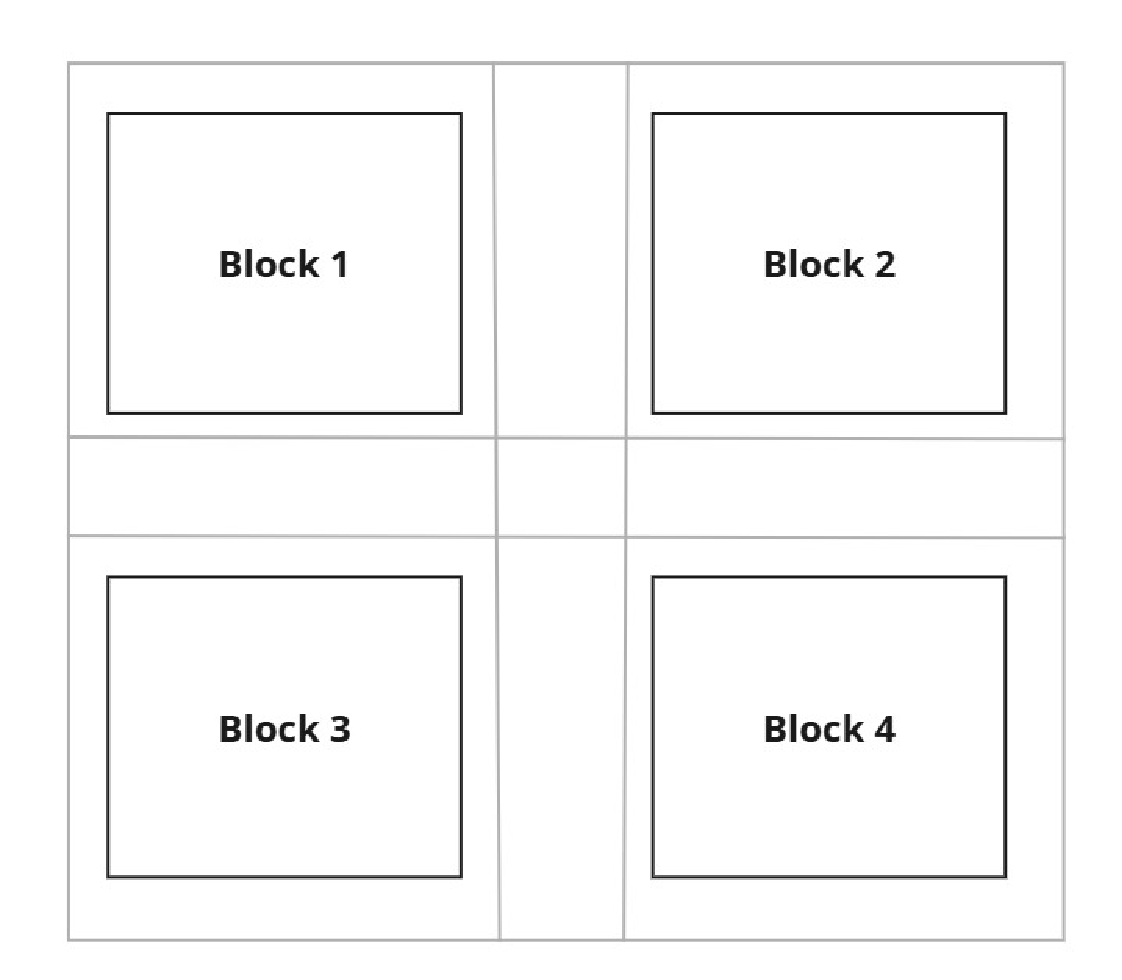
\includegraphics[width=5cm, height=5cm]{cbrp-instance.pdf}}
  \end{minipage}%
  \begin{minipage}[c]{.49\textwidth}
    \centering
    \subfloat[A spraying vehicle route covering four city blocks.]{\label{fig:route_fumace_car}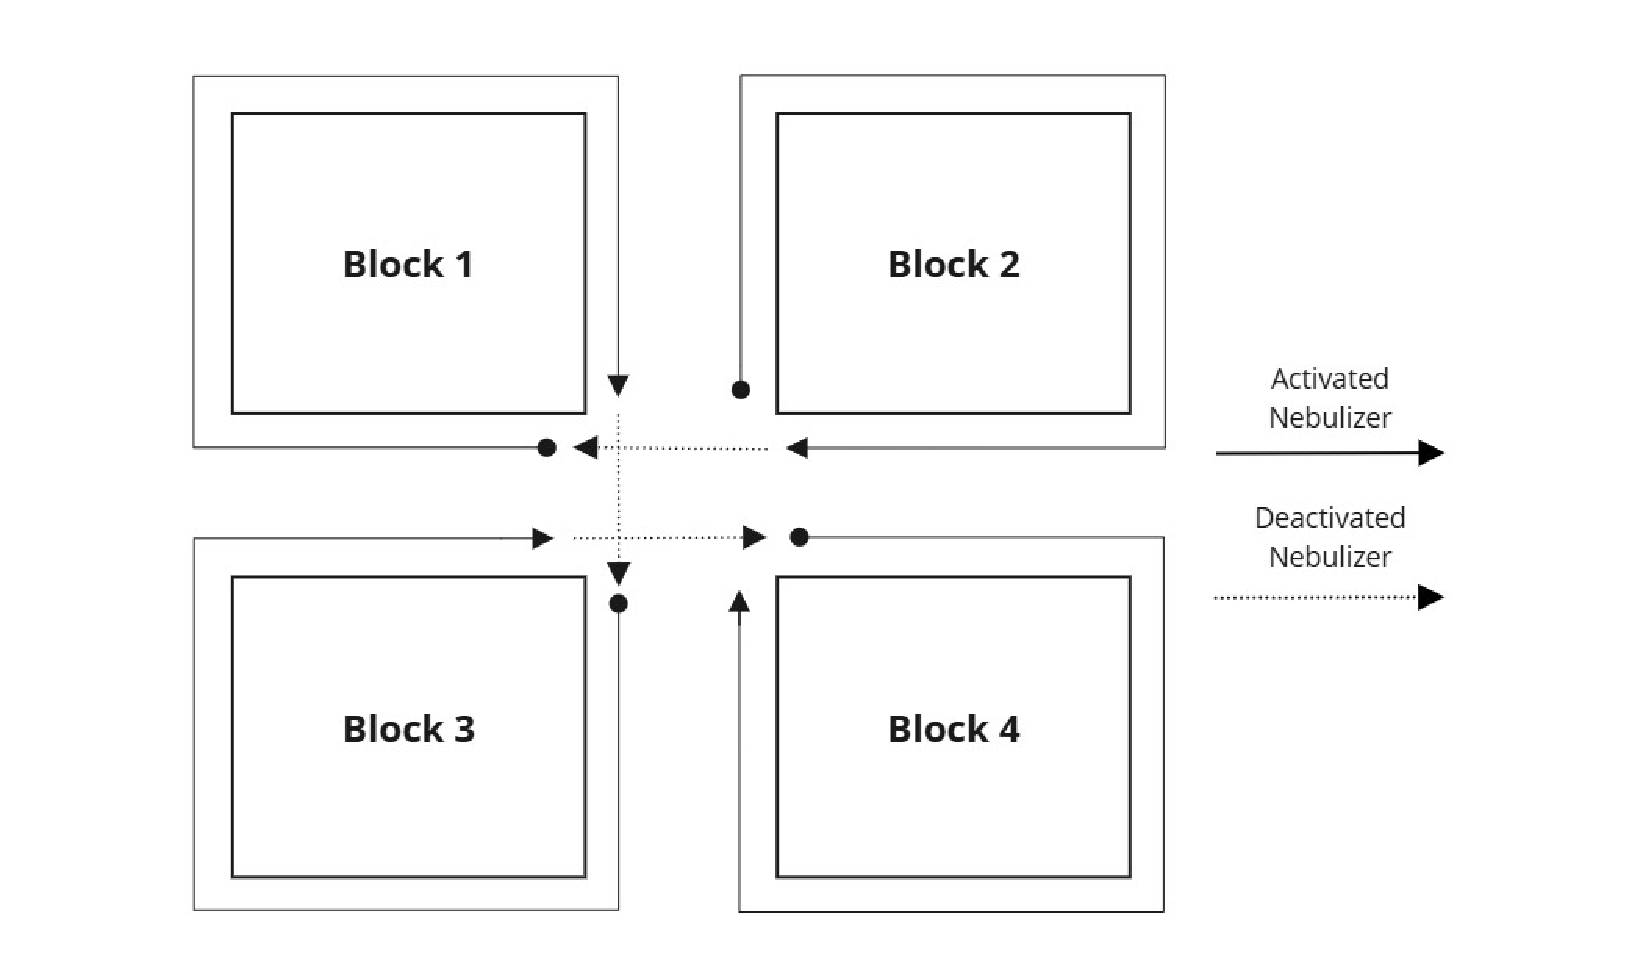
\includegraphics[width=8cm, height=5cm]{nebulizer-activated.pdf}}
  \end{minipage}
  \caption{\label{fig:route-ex} CBRP example.}
\end{figure}

The CBRP is introduced as a general framework for addressing the routing of spraying vehicles and other city block servicing problems. The objective of the CBRP is to determine an optimal traversal that services a subset of blocks within a network, maximizing the total collected benefit from each serviced block. We define the CBRP as follows. Consider a planar-oriented graph $D(V,A)$ representing a street network, where each arc $a \in A$ has a deadheading time $t_a \geqslant 0$ and a service time $t^{'}_a$ such that $t_a \leqslant t^{'}_a$. There is a set of city blocks $B = \{b : b \subseteq A\}$, where each block $b$ has an associated prize $p_b$ that can be collected by servicing all its surrounding arcs and the notation $t^{'}_b$ is used to represent the sum of the service time for all arcs $b$. A vehicle traverses the graph $D$ following a route that can serve a subset of blocks within a given time limit $T$. This work considers two types of solution routes, depending on whether the vertices can be visited more than once: \textit{Walk-based route}, in which any vertex (or arc) can be visited multiple times; and \textit{Path-based route}, in which no vertex appears more than once. An optimal route (walk or path) is one that maximizes the total prize collected from the serviced blocks while respecting the vehicle time limit $T$.

We now present key properties of the CBRP. First, we observe that once a block starts being serviced at a given node, it must be fully encircled before the vehicle moves to another block. This leads to the following properties.

\begin{property}
\label{claim:core_insight}
A block can be serviced if at least one of its nodes is visited.
\end{property}

From Property~\ref{claim:core_insight}, when formulating the problem, it is not necessary to explicitly require the vehicle to completely traverse a block's perimeter in order to count it as serviced. Instead, servicing can be achieved by visiting at least one node within the block and accounting for the corresponding service time. 

\Cref{fig:servicing_block_no_surrounding_strategy} illustrates an example of this strategy, where servicing is achieved without requiring a full traversal of the block’s perimeter.

\begin{figure}[ht!]
  \centering
  \begin{subfigure}{.3\textwidth}
    \centering
    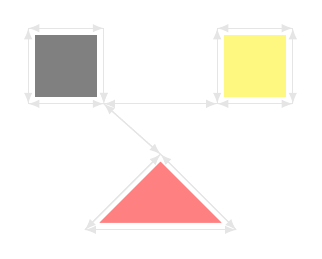
\begin{tikzpicture}[>=latex, scale=.8]
      % nodes
      % block A
      \coordinate (A1) at (3, 2);
      \coordinate (A2) at (4, 1);
      \coordinate (A3) at (2, 1);
      \coordinate (BorderA1) at (3, 2.1);
      \coordinate (BorderA2) at (4.2, 0.9);
      \coordinate (BorderA3) at (1.8, 0.9);
      % block B
      \coordinate (B1) at (2, 3);
      \coordinate (B2) at (1, 3);
      \coordinate (B3) at (1, 4);
      \coordinate (B4) at (2, 4);
      \coordinate (BorderB1) at (2.1, 2.9);
      \coordinate (BorderB2) at (0.9, 2.9);
      \coordinate (BorderB3) at (0.9, 4.1);
      \coordinate (BorderB4) at (2.1, 4.1);
      % block C
      \coordinate (C1) at (4, 3);
      \coordinate (C2) at (4, 4);
      \coordinate (C3) at (5, 4);
      \coordinate (C4) at (5, 3);
      \coordinate (BorderC1) at (3.9, 2.9);
      \coordinate (BorderC2) at (3.9, 4.1);
      \coordinate (BorderC3) at (5.1, 4.1);
      \coordinate (BorderC4) at (5.1, 2.9);
      % blocks
      \def\blockA{A1, A2, A3}
      \def\blockB{B1, B2, B3, B4}
      \def\blockC{C1, C2, C3, C4}
      % arcs
      \def\arcs{%
        BorderA1 BorderB1
        BorderB1 BorderA1
        BorderB1 BorderC1
        BorderC1 BorderB1
        % block A
        BorderA1 BorderA2
        BorderA2 BorderA1
        BorderA2 BorderA3
        BorderA3 BorderA2
        BorderA3 BorderA1
        BorderA1 BorderA3
        % block B
        BorderB1 BorderB2
        BorderB2 BorderB3
        BorderB3 BorderB4
        BorderB4 BorderB1
        BorderB2 BorderB1
        BorderB3 BorderB2
        BorderB4 BorderB3
        BorderB4 BorderB1
        % block C
        BorderC1 BorderC2
        BorderC2 BorderC3
        BorderC3 BorderC4
        BorderC4 BorderC1
        BorderC2 BorderC1
        BorderC3 BorderC2
        BorderC4 BorderC3
        BorderC1 BorderC4
      }
      \readarray\arcs\Arcs[15,2]
      % print arcs
      \drawArcs{\Arcs}{\ArcsROWS}{->, gray!20, to path={-| (\tikztotarget)}}
      % block 1
      \drawBlock{A1}{\blockA}{red!50};
      %block 2
      \drawBlock{B1}{\blockB}{black!50};
      %block 3
      \drawBlock{C1}{\blockC}{yellow!50};
    \end{tikzpicture}
    \caption{Instance example.}
    \label{fig:three_street_blocks_instance}
  \end{subfigure}
  \begin{subfigure}{.3\textwidth}
    \centering
    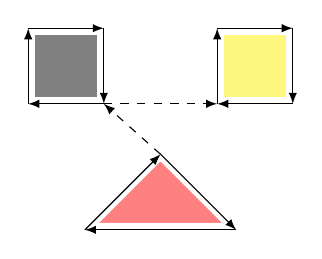
\begin{tikzpicture}[>=latex, scale=.8]
      % nodes
      % block A
      \coordinate (A1) at (3, 2);
      \coordinate (A2) at (4, 1);
      \coordinate (A3) at (2, 1);
      \coordinate (BorderA1) at (3, 2.1);
      \coordinate (BorderA2) at (4.2, 0.9);
      \coordinate (BorderA3) at (1.8, 0.9);
      % block B
      \coordinate (B1) at (2, 3);
      \coordinate (B2) at (1, 3);
      \coordinate (B3) at (1, 4);
      \coordinate (B4) at (2, 4);
      \coordinate (BorderB1) at (2.1, 2.9);
      \coordinate (BorderB2) at (0.9, 2.9);
      \coordinate (BorderB3) at (0.9, 4.1);
      \coordinate (BorderB4) at (2.1, 4.1);
      % block C
      \coordinate (C1) at (4, 3);
      \coordinate (C2) at (4, 4);
      \coordinate (C3) at (5, 4);
      \coordinate (C4) at (5, 3);
      \coordinate (BorderC1) at (3.9, 2.9);
      \coordinate (BorderC2) at (3.9, 4.1);
      \coordinate (BorderC3) at (5.1, 4.1);
      \coordinate (BorderC4) at (5.1, 2.9);
      % blocks
      \def\blockA{A1, A2, A3}
      \def\blockB{B1, B2, B3, B4}
      \def\blockC{C1, C2, C3, C4}
      % arcs
      \def\nonSprayingArcs{%
        BorderA1 BorderB1
        BorderB1 BorderC1
      }
      \readarray\nonSprayingArcs\NonSprayingArcs[2,2]
      % spraying arcs
      \def\arcsSpraying{%
        % block A
        BorderA1 BorderA2
        BorderA2 BorderA3
        BorderA3 BorderA1
        % block B
        BorderB1 BorderB2
        BorderB2 BorderB3
        BorderB3 BorderB4
        BorderB4 BorderB1
        % block C
        BorderC1 BorderC2
        BorderC2 BorderC3
        BorderC3 BorderC4
        BorderC4 BorderC1
      }
      \readarray\arcsSpraying\ArcsSpraying[11,2]
      % print arcs
      \drawArcs{\NonSprayingArcs}{\NonSprayingArcsROWS}{dashed, ->}
      \drawArcs{\ArcsSpraying}{\ArcsSprayingROWS}{->, to path={-| (\tikztotarget)}}
      % block 1
      \drawBlock{A1}{\blockA}{red!50};
      %block 2
      \drawBlock{B1}{\blockB}{black!50};
      %block 3
      \drawBlock{C1}{\blockC}{yellow!50};
      %lines
      % \filldraw[black] (BorderA1) circle (1pt);
    \end{tikzpicture}
    \caption{Explicit block servicing.}
    \label{fig:three_street_blocks_route_surrounding}
  \end{subfigure}
  \begin{subfigure}{.3\textwidth}
    \centering
    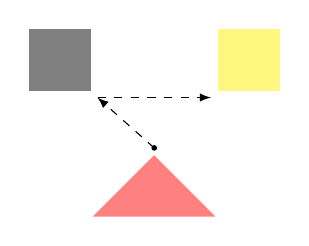
\begin{tikzpicture}[>=latex, scale=.8]
      % nodes
      % block A
      \coordinate (A1) at (3, 2);
      \coordinate (A2) at (4, 1);
      \coordinate (A3) at (2, 1);
      \coordinate (BorderA1) at (3, 2.1);
      \coordinate (BorderA2) at (4.2, 0.9);
      \coordinate (BorderA3) at (1.8, 0.9);
      % block B
      \coordinate (B1) at (2, 3);
      \coordinate (B2) at (1, 3);
      \coordinate (B3) at (1, 4);
      \coordinate (B4) at (2, 4);
      \coordinate (BorderB1) at (2.1, 2.9);
      \coordinate (BorderB2) at (0.9, 2.9);
      \coordinate (BorderB3) at (0.9, 4.1);
      \coordinate (BorderB4) at (2.1, 4.1);
      % block C
      \coordinate (C1) at (4, 3);
      \coordinate (C2) at (4, 4);
      \coordinate (C3) at (5, 4);
      \coordinate (C4) at (5, 3);
      \coordinate (BorderC1) at (3.9, 2.9);
      \coordinate (BorderC2) at (3.9, 4.1);
      \coordinate (BorderC3) at (5.1, 4.1);
      \coordinate (BorderC4) at (5.1, 2.9);
      % blocks
      \def\blockA{A1, A2, A3}
      \def\blockB{B1, B2, B3, B4}
      \def\blockC{C1, C2, C3, C4}
      % arcs
      \def\arcs{%
        BorderA1 BorderB1
        BorderB1 BorderC1
      }
      \readarray\arcs\Arcs[2,2]
      % print arcs
      \drawArcs{\Arcs}{\ArcsROWS}{dashed, ->}
      % block 1
      \drawBlock{A1}{\blockA}{red!50};
      %block 2
      \drawBlock{B1}{\blockB}{black!50};
      %block 3
      \drawBlock{C1}{\blockC}{yellow!50};
      %lines
      \filldraw[black] (BorderA1) circle (1pt);
    \end{tikzpicture}
    \caption{Implicit block servicing.}
    \label{fig:three_street_blocks_route_one_node_visit}
  \end{subfigure}
  \caption{Strategies for servicing blocks.}
  \label{fig:servicing_block_no_surrounding_strategy}
\end{figure}


Assuming the implicit servicing of a block as allowed by Property~\ref{claim:core_insight}, additional properties can be established concerning optimal solutions. Let $V_B = \bigcup_{b \in B} V(b)$ be the set of nodes belonging to some city block, and let $S^{*} = (v_1, ..., v_n)$ represent an optimal route.

% \chapter{Mathematical Models} \label{chapter:models}

Since routes may start and end at different nodes of $D$, we augment the digraph to $D' = (V', A')$  to include a dummy depot $0$ and a set of arcs such that $A' = \{(0, u), (u, 0)\}$, and $t_{u0} = t_{0u} = 0$, $\forall u \in V$. Consider $B(i)$ as the set of blocks touching node $i$, $V(b)$ as the set of vertices in block $b$, and the following sets of variables:

 \section{Model Without repeating Nodes}
 
\begin{itemize}
  \item $x_{ij}$: binary variable that indicates whether arc $(i, j) \in
    A'$ belongs to the route ($x_{ij} = 1$) or not ($x_{ij} = 0$);
  \item $y_{ib}$: binary variable that is valued 1 if node $i \in V$ is
    used as the starting point to service block $b \in B(i)$, and valued 0 otherwise; 
\end{itemize}

With these variables, the T-CBRP formulation reads:
\allowdisplaybreaks
\begin{align}
  \text{(T-CBRP) } & \max \sum_{i \in V} \sum_{b \in B} p_b y_{ib} & \label{eq:of}\\
  \nonumber \text{subject to:} & & \\
       & \sum_{a \in \delta^{-}(0)} x_{a} = \sum_{a' \in \delta^{+}(0)} x_{a'} = 1 & \label{eq:s-t-all} \\
       %
       & \sum_{a \in \delta^{-}(i)} x_{a} - \sum_{a' \in \delta^{+}(i)} x_{a'} = 0 & \ \forall i \in V \label{eq:flow-conservation} \\
       % & \sum_{i \in V'} \sum_{b \in B} f^I_b y_{ib} \leq I_{\max} & \label{eq:max-insecticide} \\
       %
       & \sum_{i \in V(b)} y_{ib} \leq 1 & \ \forall b \in B \label{eq:max-attend} \\
       %
       & \sum_{a \in \delta^{+}(i)} x_{a} \geq y_{ib} & \ \forall i \in V(b), b \in B \label{eq:in-path} \\
       %
       & \sum_{a \in A'} x_{a}t_{a} + \sum_{i \in V'} \sum_{b \in B} y_{ib}t_{b} \leq T & \label{eq:max-time} \\
       %
       & \sum_{a \in A(S)} x_{a} \leq |V(S)| - 1 & \ \forall S \subseteq V \label{eq:circuit-subtour-elimination} \\
       %
       & x \in \mathbb{B}^{|A'|} & \label{eq:dom-x} \\
       & y \in \mathbb{B}^{|V'| * |B|} & \label{eq:dom-y}
\end{align}

The T-CBRP formulation generates a tour that starts and ends at the dummy depot. The objective function~\eqref{eq:of} maximizes the profit collected from each block. Constraints~\eqref{eq:s-t-all}-\eqref{eq:flow-conservation} enforce flow conservation in each node. Constraints~\eqref{eq:max-attend} and~\eqref{eq:in-path} ensure that only one node is used as the starting point for servicing a block. Constraints~\eqref{eq:max-time} limit the time used by the route, considering different times whether the vehicle is servicing or not. Constraints~\eqref{eq:circuit-subtour-elimination} eliminate subcycles. Constraints~\eqref{eq:dom-x}-\eqref{eq:dom-y} define the domain of the variables.

The subcycle elimination constraints, exponentially large in the size of the input, 
can be replaced by the compact set of variables and constraints known as MTZ (Miller-Tucker-Zemlin). To this end, consider the following variables:

\begin{itemize}
    \item $w_{a}$: real variable representing the accumulated time in arc $a \in A'$.
\end{itemize}

Now it is possible to replace constraints \eqref{eq:circuit-subtour-elimination} with the following:

\begin{align}
  & w_{a'} \geq w_{a} + x_{a}t_{a} - (2 - x_{a'} - x_{a})T & \ \forall a \in \delta^{+}(i), a' \in \delta^{-}(i), i \in V' \label{eq:max-time-compact-leq} \\
   %
   & w_{a} \leq T & \ \forall a \in \delta^{+}(0) & \label{eq:max-time-compact}
\end{align}

Constraints~\eqref{eq:max-time-compact-leq} compute the accumulated time for each arc while  Constraints~\eqref{eq:max-time-compact} limit the amount of time used in the route. This new formulation has a number of constraints that grows polynomially with the size of the instance and the resulting route is equivalent to the formulation T-CBRP, i.e., a closed path.

\section{Models That Allows Repetitions os Arcs}

The first option is to use the above models with a new Graph create from the transitive closure of D.

The second options is to use the plannar input graph with the following model:

\begin{itemize}
  \item $x_{ij}$: integer variable that count how many times the arc $(i, j) \in A'$ was traveled in the route;
  \item $y_{b}$: binary variable that is valued 1 if block $b \in B(i)$ is serviced, and valued 0 otherwise; 
\end{itemize}

\begin{align}
  \text{(W-CBRP) } & \max \sum_{i \in V} \sum_{b \in B} p_b y_{b} & \label{eq:of}\\
  \nonumber \text{subject to:} & & \\
       & \sum_{a \in \delta^{-}(0)} x_{a} = \sum_{a' \in \delta^{+}(0)} x_{a'} = 1 & \label{eq:s-t-all} \\
       %
       & \sum_{a \in \delta^{-}(i)} x_{a} - \sum_{a' \in \delta^{+}(i)} x_{a'} = 0 & \ \forall i \in V \label{eq:flow-conservation} \\
       % & \sum_{i \in V'} \sum_{b \in B} f^I_b y_{ib} \leq I_{\max} & \label{eq:max-insecticide} \\
       %
       % & \sum_{i \in V(b)} y_{ib} \leq 1 & \ \forall b \in B \label{eq:max-attend} \\
       %
       & \sum_{a \in \delta^{+}(i)} x_{a} \geq y_{b} & \ \forall i \in V(b), b \in B \label{eq:in-path} \\
       %
       & \sum_{a \in A'} x_{a}t_{a} + \sum_{b \in B} y_{b}t_{b} \leq T & \label{eq:max-time} \\
       %
       & \sum_{a \in A(S)} x_{a} \leq |V(S)| - 1 + \sum_{a' \in \delta^{+}(S)} x_{a'} & \ \forall S \subseteq V \label{eq:new-walk-subtour-elimination} \\
       %
       & x \in \mathbb{Z}^{|A'|} & \label{eq:dom-x} \\
       & y \in \mathbb{B}^{|B|} & \label{eq:dom-y}
\end{align}


% \chapter{Heuristics}

\section{Constructive Heuristic}

How to connect blocks:

\begin{figure}[ht!]
  \centering
  \begin{subfigure}{0.49\textwidth}
      \centering
      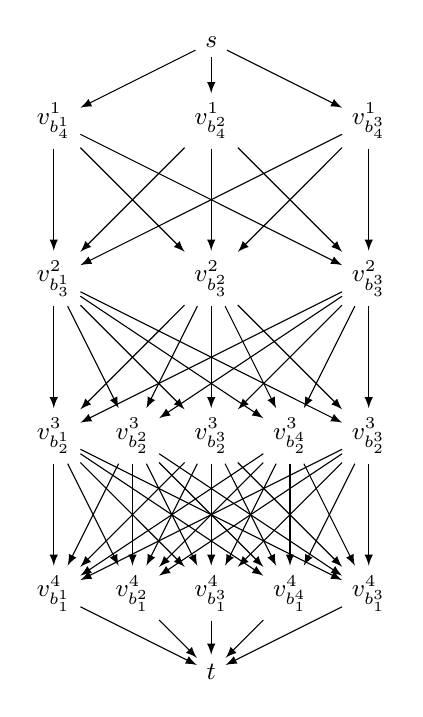
\begin{tikzpicture}[>=latex]
        \coordinate (s) at (2, 5);
        \coordinate (v11) at (0, 4);
        \coordinate (v12) at (2, 4);
        \coordinate (v13) at (4, 4);
        \coordinate (v21) at (0, 2);
        \coordinate (v22) at (2, 2);
        \coordinate (v23) at (4, 2);
        \coordinate (v31) at (0, 0);
        \coordinate (v32) at (1, 0);
        \coordinate (v33) at (2, 0);
        \coordinate (v34) at (3, 0);
        \coordinate (v35) at (4, 0);
        \coordinate (v41) at (0, -2);
        \coordinate (v42) at (1, -2);
        \coordinate (v43) at (2, -2);
        \coordinate (v44) at (3, -2);
        \coordinate (v45) at (4, -2);
        \coordinate (t)   at (2, -3);
        \node (ns)   at (s)   {\small$s$};
        \node (nv11) at (v11) {\small$v^1_{b_4^1}$};
        \node (nv12)  at (v12) {\small$v^1_{b_4^2}$};
        \node (nv13)  at (v13) {\small$v^1_{b_4^3}$};
        \node (nv21)  at (v21) {\small$v^2_{b_3^1}$};
        \node (nv22)  at (v22) {\small$v^2_{b_3^2}$};
        \node (nv23)  at (v23) {\small$v^2_{b_3^3}$};
        \node (nv31)  at (v31) {\small$v^3_{b_2^1}$};
        \node (nv32)  at (v32) {\small$v^3_{b_2^2}$};
        \node (nv33)  at (v33) {\small$v^3_{b_2^3}$};
        \node (nv34)  at (v34) {\small$v^3_{b_2^4}$};
        \node (nv35)  at (v35) {\small$v^3_{b_2^3}$};
        \node (nv41)  at (v41) {\small$v^4_{b_1^1}$};
        \node (nv42)  at (v42) {\small$v^4_{b_1^2}$};
        \node (nv43)  at (v43) {\small$v^4_{b_1^3}$};
        \node (nv44)  at (v44) {\small$v^4_{b_1^4}$};
        \node (nv45)  at (v45) {\small$v^4_{b_1^3}$};
        \node (nt)    at (t)   {\small$t$};
        % arcs
        \def\arcs{%
          ns nv11
          ns nv12
          ns nv13
          nv11 nv21
          nv11 nv22
          nv11 nv23
          nv12 nv21
          nv12 nv22
          nv12 nv23
          nv13 nv21
          nv13 nv22
          nv13 nv23
          nv21 nv31
          nv21 nv32
          nv21 nv33
          nv21 nv34
          nv21 nv35
          nv22 nv31
          nv22 nv32
          nv22 nv33
          nv22 nv34
          nv22 nv35
          nv23 nv31
          nv23 nv32
          nv23 nv33
          nv23 nv34
          nv23 nv35
          nv31 nv41
          nv31 nv42
          nv31 nv43
          nv31 nv44
          nv31 nv45
          nv32 nv41
          nv32 nv42
          nv32 nv43
          nv32 nv44
          nv32 nv45
          nv33 nv41
          nv33 nv42
          nv33 nv43
          nv33 nv44
          nv33 nv45
          nv34 nv41
          nv34 nv42
          nv34 nv43
          nv34 nv44
          nv34 nv45
          nv35 nv41
          nv35 nv42
          nv35 nv43
          nv35 nv44
          nv35 nv45
          nv41 nt
          nv42 nt
          nv43 nt
          nv44 nt
          nv45 nt
        }
        \readarray\arcs\Arcs[9,2]
        % print arcs
        \drawArcs{\Arcs}{\ArcsROWS}{->}
      \end{tikzpicture}
      \caption{$D^G$ example.}
  \end{subfigure}
  \begin{subfigure}{0.49\textwidth}
      \centering
      \begin{tikzpicture}[>=latex]
        \coordinate (s) at (2, 5);
        \coordinate (v11) at (0, 4);
        \coordinate (v12) at (2, 4);
        \coordinate (v13) at (4, 4);
        \coordinate (v21) at (0, 2);
        \coordinate (v22) at (2, 2);
        \coordinate (v23) at (4, 2);
        \coordinate (v31) at (0, 0);
        \coordinate (v32) at (1, 0);
        \coordinate (v33) at (2, 0);
        \coordinate (v34) at (3, 0);
        \coordinate (v35) at (4, 0);
        \coordinate (v41) at (0, -2);
        \coordinate (v42) at (1, -2);
        \coordinate (v43) at (2, -2);
        \coordinate (v44) at (3, -2);
        \coordinate (v45) at (4, -2);
        \coordinate (t)   at (2, -3);
        \node (ns)   at (s)   {\small$s$};
        \node (nv11) at (v11) {\small$v^1_{b_4^1}$};
        \node (nv12)  at (v12) {\small$v^1_{b_4^2}$};
        \node (nv13)  at (v13) {\small$v^1_{b_4^3}$};
        \node (nv21)  at (v21) {\small$v^2_{b_3^1}$};
        \node (nv22)  at (v22) {\small$v^2_{b_3^2}$};
        \node (nv23)  at (v23) {\small$v^2_{b_3^3}$};
        \node (nv31)  at (v31) {\small$v^3_{b_2^1}$};
        \node (nv32)  at (v32) {\small$v^3_{b_2^2}$};
        \node (nv33)  at (v33) {\small$v^3_{b_2^3}$};
        \node (nv34)  at (v34) {\small$v^3_{b_2^4}$};
        \node (nv35)  at (v35) {\small$v^3_{b_2^3}$};
        \node (nv41)  at (v41) {\small$v^4_{b_1^1}$};
        \node (nv42)  at (v42) {\small$v^4_{b_1^2}$};
        \node (nv43)  at (v43) {\small$v^4_{b_1^3}$};
        \node (nv44)  at (v44) {\small$v^4_{b_1^4}$};
        \node (nv45)  at (v45) {\small$v^4_{b_1^3}$};
        \node (nt)    at (t)   {\small$t$};
        % arcs
        \def\arcs{%
          nv11 nv23
          nv23 nv32
        }
        \readarray\arcs\Arcs[9,2]
        % print arcs
        \drawArcs{\Arcs}{\ArcsROWS}{->}
      \end{tikzpicture}
      \caption{Obtained tour with $k = 3$.}
  \end{subfigure}
  \caption{Block connection heuristic.}
  \label{fig:brkga_example}
\end{figure}

% \begin{algorithm}[!ht]
% \scriptsize
% % \DontPrintSemicolon 
% 	\caption{\label{alg:stochastic-construction} Stochastic Initial Solution}
% 	\KwIn{Graph G, Scenarios S, Time T}
% 	\KwOut{$X, Y$ set of |S| routes and their respective attended blocks}

%     $P_0 \leftarrow$ update profits from first stage\;
%     $T_{UB} = 1.0 * T$\;
%     $T_{LB} = 0.5 * T$\;
    
% 	\Repeat{close the gap between $T_{UB}$ and $T_{LB}$}{ \label{line:rep-beg} 
%         $T' \leftarrow $ reserved time to attend (from binary search)\; 
%         $Y_0, X_0 \leftarrow$ solve first stage route ($P_0, T'$)\;

%         \For{$s = 1, 2, \dots, |S|$}{
%             $P_s \leftarrow$ update second stage profit $(Y_0)$\;
%             $Y_s, X_s \leftarrow$ solve second stage route ($P_s, T'$)\;
%             $C_k(x) \leftarrow 0$\; 
%             \For{$j = 1, 2, \dots, n$}{
%                 \uIf{$k \neq j$}{
%                    $C_k(x) \leftarrow C_k(x) + (c_{kj} * x_j)$\;
%                 }
%             } \label{line:calc-ckx-end}
            
%            \uIf{$C_k(x) < C_k/2$ \textbf{and} $x_k = 0$}{\label{line:if-change}
%                 $x_k \leftarrow 1$\;
%             } 
%             \uElseIf {$C_k(x) > C_k/2$ \textbf{and} $x_k = 1$} {
%               $x_k \leftarrow 0$\;
%             } \label{line:if-change-two}
%         }
% 	} \label{line:rep-end}
% 	\Return{$x$}\;

% \end{algorithm}

% O corpo da dissertação ou tese começa aqui:
% \chapter{Introdução}

% Lorem ipsum dolor sit amet, consectetur adipiscing elit, sed do eiusmod
% tempor incididunt ut labore et dolore magna aliqua. Ut enim ad minim
% veniam, quis nostrud exercitation ullamco laboris nisi ut aliquip ex ea
% commodo consequat. Duis aute irure dolor in reprehenderit in voluptate
% velit esse cillum dolore eu fugiat nulla pariatur. Excepteur sint occaecat
% cupidatat non proident, sunt in culpa qui officia deserunt mollit anim id
% est laborum.

% \begin{table}
% \caption[Shorter table caption]{Table caption caption caption caption
%   caption caption caption caption caption caption caption caption caption
%   caption caption caption caption caption caption caption caption caption
%   caption caption.}
% \label{t:label0}
% \begin{center}
% \begin{tabular}{|c|c|}
% \hline
% a & b \\\hline
% c & d \\\hline
% \end{tabular}
% \end{center}
% \end{table}

% Lorem ipsum dolor sit amet, consectetur adipiscing elit, sed do eiusmod
% tempor incididunt ut labore et dolore magna aliqua. Ut enim ad minim
% veniam, quis nostrud exercitation ullamco laboris nisi ut aliquip ex ea
% commodo consequat. Duis aute irure dolor in reprehenderit in voluptate
% velit esse cillum dolore eu fugiat nulla pariatur. Excepteur sint occaecat
% cupidatat non proident, sunt in culpa qui officia deserunt mollit anim id
% est laborum.

% Lorem ipsum dolor sit amet, consectetur adipiscing elit, sed do eiusmod
% tempor incididunt ut labore et dolore magna aliqua. Ut enim ad minim
% veniam, quis nostrud exercitation ullamco laboris nisi ut aliquip ex ea
% commodo consequat. Duis aute irure dolor in reprehenderit in voluptate
% velit esse cillum dolore eu fugiat nulla pariatur. Excepteur sint occaecat
% cupidatat non proident, sunt in culpa qui officia deserunt mollit anim id
% est laborum.

% Lorem ipsum dolor sit amet, consectetur adipiscing elit, sed do eiusmod
% tempor incididunt ut labore et dolore magna aliqua. Ut enim ad minim
% veniam, quis nostrud exercitation ullamco laboris nisi ut aliquip ex ea
% commodo consequat. Duis aute irure dolor in reprehenderit in voluptate
% velit esse cillum dolore eu fugiat nulla pariatur. Excepteur sint occaecat
% cupidatat non proident, sunt in culpa qui officia deserunt mollit anim id
% est laborum.

% Lorem ipsum dolor sit amet, consectetur adipiscing elit, sed do eiusmod
% tempor incididunt ut labore et dolore magna aliqua. Ut enim ad minim
% veniam, quis nostrud exercitation ullamco laboris nisi ut aliquip ex ea
% commodo consequat. Duis aute irure dolor in reprehenderit in voluptate
% velit esse cillum dolore eu fugiat nulla pariatur. Excepteur sint occaecat
% cupidatat non proident, sunt in culpa qui officia deserunt mollit anim id
% est laborum~\cite{2014-bic,2015-ela}.

% \begin{figure}
% \centerline{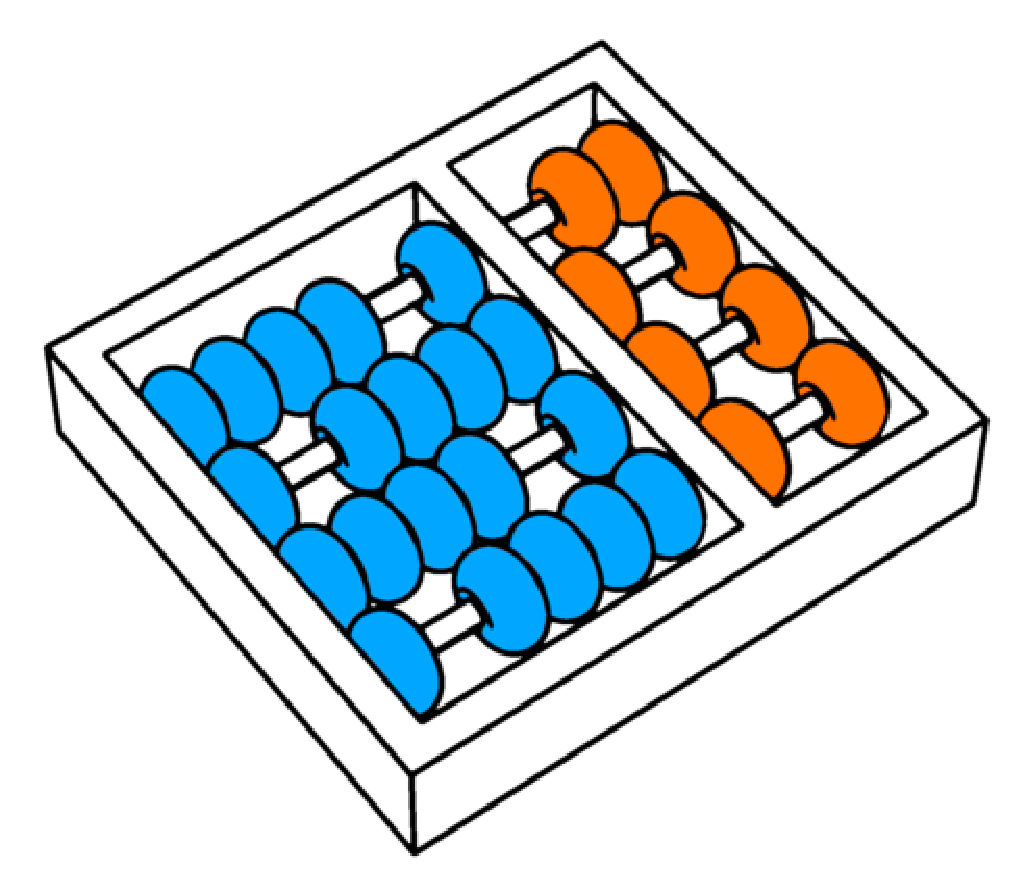
\includegraphics[scale=0.2]{logo-ic-unicamp.eps}}
% \caption[Shorter figure caption]{Figure Caption caption caption caption
%   caption caption caption caption caption caption caption caption caption
%   caption caption caption caption caption caption caption caption caption
%   caption caption.}
% \label{f:label1}
% \end{figure}

% Lorem ipsum dolor sit amet, consectetur adipiscing elit, sed do eiusmod
% tempor incididunt ut labore et dolore magna aliqua. Ut enim ad minim
% veniam, quis nostrud exercitation ullamco laboris nisi ut aliquip ex ea
% commodo consequat\footnote{Footnote footnote footnote footnote footnote
%   footnote footnote footnote footnote footnote footnote footnote footnote
%   footnote footnote footnote.}.  Duis aute irure dolor in reprehenderit in
% voluptate velit esse cillum dolore eu fugiat nulla pariatur. Excepteur sint
% occaecat cupidatat non proident, sunt in culpa qui officia deserunt mollit
% anim id est laborum.


% \chapter{Hipóteses}


% \chapter{Resultados}


% \chapter{Conclusões}



% As referências:
\bibliographystyle{plain}
\bibliography{ic-tese-v3}


% Os anexos, se houver, vêm depois das referências:
% \appendix
% \chapter{Anexo 1}
% \chapter{Anexo 2}

\end{document}
